\section{Introduction}
\label{sec:intro}
Humans posses an innate ability to perceive, track and interpret motion, spatial and temporal changes, ~\cite{DeFreitas2016Tracking, Marr1981Directional} enable rich interpretations of complex dynamic events from both egocentric and allocentric perspectives \cite{Burgess2006Spatial}. When observing an object move, we can inherently process any changes such as lateral shifts, rotational directions and periodic or repeated actions unfolding along a specific trajectory \cite{Burgess2006Spatial}. These sophisticated perceptual abilities are a product of our spatiotemporal cognition~\cite{Freyd1984Representational}, and form an essential foundation that allows us to comprehend and reason about physical phenomena, object interactions and causal relationships within our environment. ~\cite{Leslie1984Spatiotemporal, Johansson1973Visual}

Vision-language models (VLMs), which can also potentially perceive the motions and spatialtemporal changes in videos, constitute a prominent class of methods designed to emulate or surpass human capabilities in integrated visual and linguistic reasoning~\cite{LeCun1989Backpropagation, Dosovitskiy2021An}. While prior work has focused on static visual understanding from mass training corpuses of language and visual data~\cite{Radford2021Learning} or understanding video such as captioning~\cite{Lu2019ViLBERTPT} and scene understanding~\cite{Chen_2022_CVPR}, we find that the exceptional performance in the prior mentioned tasks does not innately carry over to spatiotemporal capabilities. This limitation is notable given that contemporary state-of-the-art VLMs are typically trained on datasets comprising of billions of annotated video-text pairs~\cite{liu2023world}. In contrast, human infants naturally develop robust spatiotemporal cognition within the first few months of life~\cite{Spelke2007Core}. Another key challenge that inhibits VLM performance in spatiotemporal tasks is the necessity to implicitly or explicitly reconstruct a four-dimensional (4D) representation of dynamic scenes and subsequently reason over such reconstruction~\cite{wang2024compositional}. As illustrated in \cref{fig:teaser}, the car is advancing forwards and turning to the left in its own frame of reference. However, from the camera's perspective, its motion appears as a combination of heading to the right and receding into the distance despite the car being in the center of the frame due to camera view rotation. Human observers can seamlessly disentangle these complex dynamics, accurately interpreting trajectories by synthesizing diverse visual cues including camera rotation compensation, stationary scene landmarks, prior knowledge of 3D and 4D environmental structures, and perspective projections \cite{Marr1981Directional,Burgess2006Spatial,Leslie1984Spatiotemporal,Freyd1984Representational}. The inability of current VLMs to similarly integrate these cues underscores an important gap. Furthermore, bridging this gap will require VLMs to develop more sophisticated mechanisms for reconstructing and reasoning over dynamic scenes, potentially drawing on  insights from cognitive science and neuroscience on how humans process and integrate spatial and temporal information.
\begin{figure}[t]
    \centering
    % Replace 'example-image' with your image file name (e.g., 'myfigure.png')
    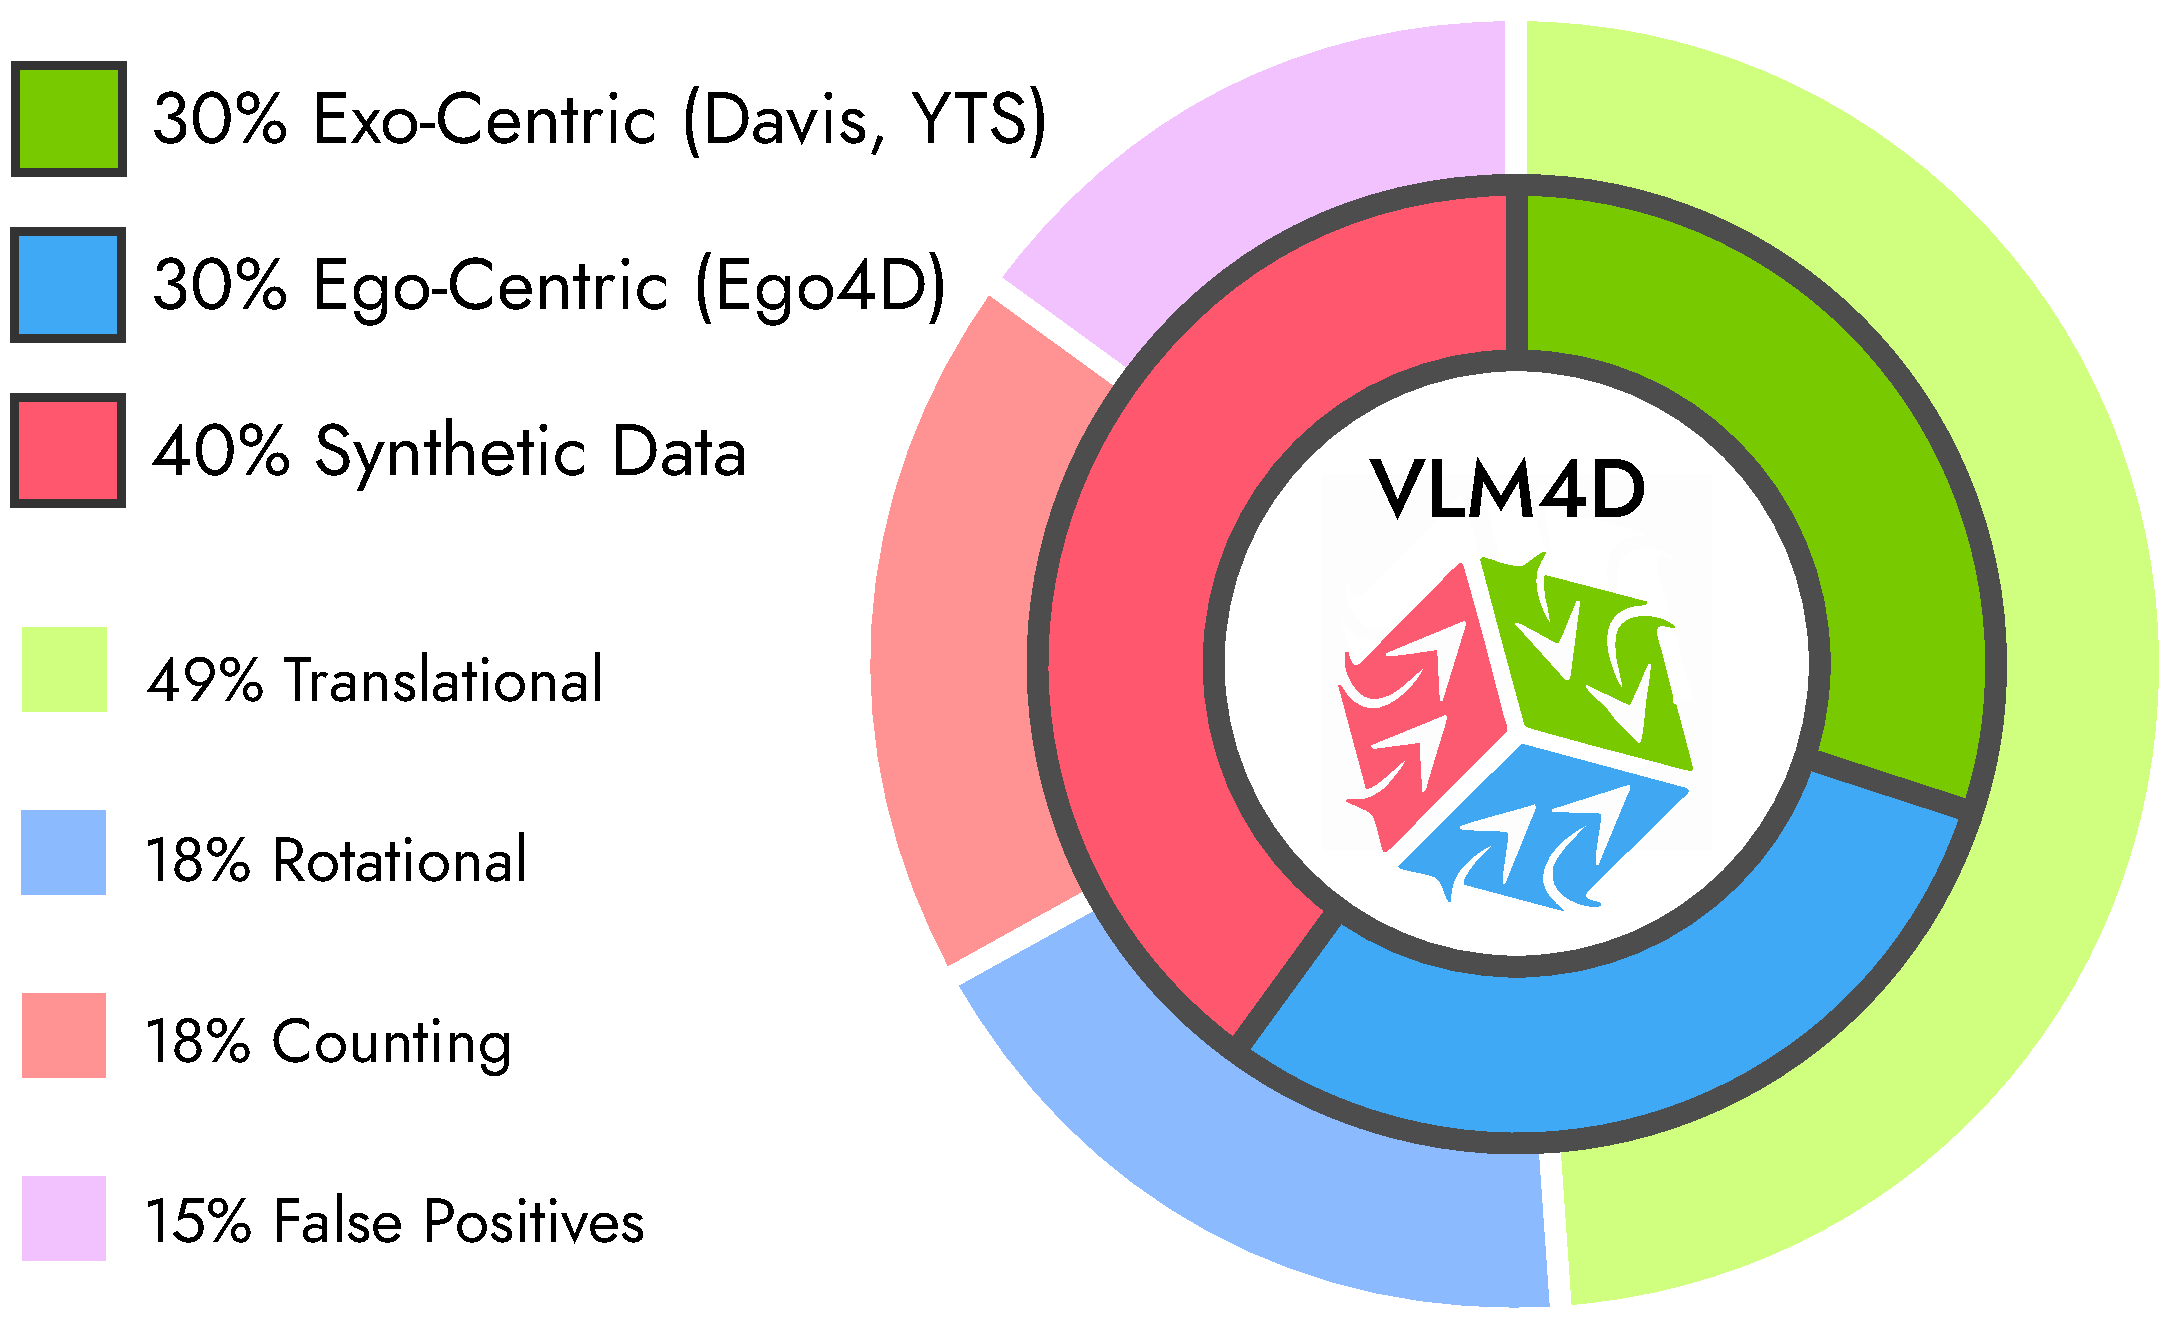
\includegraphics[width=0.45\textwidth]{figures/piechart_dataset_stats.pdf}
    \caption{\textbf{Distribution of Dataset Sources and Annotations.} Breakdown of our dataset illustrating the proportions of data sourced from third-person (Davis, YouTube), first-person (Ego4D), and synthetic data, categorized by annotation types: translational, rotational, action, counting, and false positives.}
    \label{fig:data_piechart}
    \vspace{-0.3cm}
\end{figure}

\begin{figure*}[ht]
    \centering
    % Replace 'example-image' with your image file name (e.g., 'myfigure.png')
    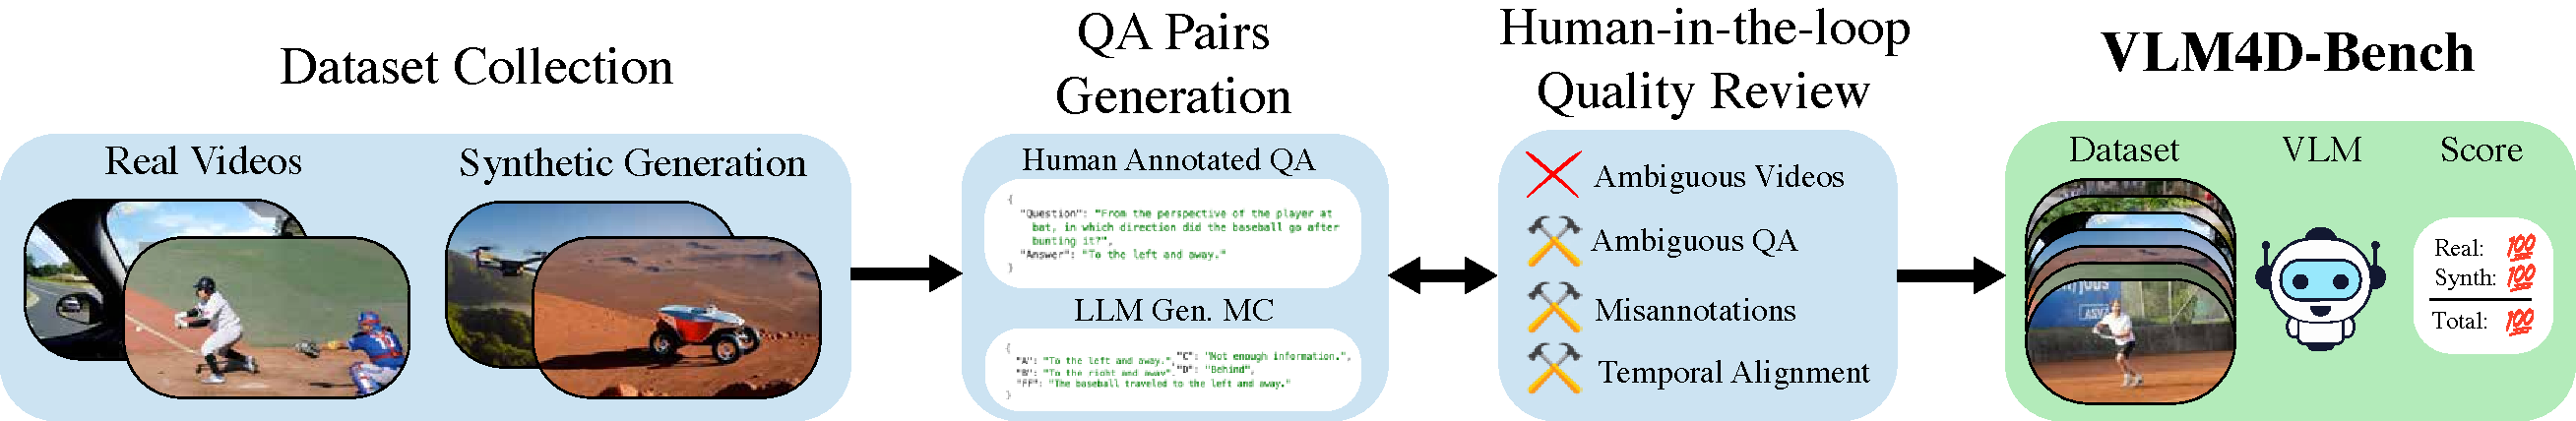
\includegraphics[width=1\textwidth]{figures/dataset_generation_v2.pdf}
    \caption{\textbf{Dataset Generation and Annotation Pipeline.} Our dataset was constructed by collecting real videos and generating synthetic data, followed by human-in-the-loop quality reviews to address ambiguous videos and annotations. After temporal alignment and quality assurance, human-annotated questions and answers were created, complemented by multiple-choice questions generated by large language models (LLMs). The final dataset includes real-world and synthetic video data with comprehensive VLM scoring metrics.}
    \label{fig:dataset_pipeline}
    \vspace{-0.4cm}
\end{figure*}

With the mentioned limitations of exisiting VLMs, to effectively characterize and challenge the existing spatiotemporal reasoning abilities of VLMs, we directly evaluate their capacity to track complex directional movements and perspective transformations over time. We introduce \texttt{VLM4D}, a rigorous benchmark specifically designed to probe the spatiotemporal grounding capabilities of current vision-language models. Through this contribution, we aim to catalyze research that addresses the critical gap in spatiotemporal understanding and reasoning within VLMs and provide a foundational analysis highlighting key deficiencies in existing models. 

We summarize our main~\textbf{contributions} as follows:
\begin{enumerate}
\item We propose the first benchmark~\texttt{VLM4D} explicitly designed to rigorously evaluate the spatiotemporal reasoning capabilities of Vision-Language Models (VLMs).
\item We introduce a novel, meticulously curated dataset consisting of diverse real-world and synthetic video sequences paired with carefully crafted spatiotemporal question-answer (QA) annotations.
\item We conduct an analysis to identify critical limitations in the spatiotemporal reasoning performance of contemporary VLMs, highlighting fundamental challenges and charting clear directions for impactful future research.
\end{enumerate}





